\chapter{Einleitung}

Im Rahmen des Moduls \glqq Advanced Software Engineering\grqq{} wurde ein Schachspiel als Projektgrundlage ausgewählt. 
Chess of Duty ist ein Offline-Multiplayer-Schachspiel für zwei Personen. 
Das Hauptziel des Programmentwurfs besteht darin, Schach gemäß den Standardregeln zu implementieren. 

Der Nutzen des Schachspiels für unsere Kunden entspricht dem von anderen Videospielen. 
Die Anwendung dient ausschließlich der Unterhaltung der Nutzer. 
Zusätzlich können die Anwender ihre strategischen Fähigkeiten und logisches Denken trainieren.

Das Schachspiel wird objektorientiert konzipiert und in Processing programmiert. 
Processing ist eine Open-Source-Programmiersprache, die auf Java basiert und einen besonderen Schwerpunkt auf die einfache Erstellung von Grafiken und Animationen setzt. 
Dadurch eignet sich Processing besonders für die Gestaltung interaktiver Benutzeroberflächen. 

\begin{balken}
    \tip
    \\
    Das GitHub-Repository ist mit folgendem Link erreichbar:\\
    \url{https://github.com/clemens1403/AdvSWE}
\end{balken}

\section{Vorwort}

Sehr geehrter Herr Lindner, anbei finden Sie unsere Ausarbeitung für den Programmentwurf aus dem fünften und sechsten Semester. 
Während der Projektarbeit sind verschiedene Herausforderungen aufgetreten, insbesondere bei der Projektwahl und der Auswahl des Technologiestacks. 
Für die Umsetzung einer Clean Architecture hätte sich im Nachhinein ein Verwaltungsprogramm als geeigneter erwiesen. 
Zudem gestaltete sich die Verwendung von Processing in einem Java-Projekt leider weniger intuitiv als von den Entwicklern angenommen. 
Insbesondere die Integration von Processing in IntelliJ bereitete längere Zeit Probleme.

Trotz dieser Schwierigkeiten ist das Ergebnis des Programmentwurfs ein Projekt, das die in der Vorlesung vermittelten Methoden und Prinzipien bestmöglich umsetzt. 
Sollte etwas nicht umgesetzt worden sein, wird darauf zumindest eingegangen. 

Die Implementierung der Schachlogik war äußerst umfangreich, weshalb einige Funktionen nicht unterstützt werden, beispielsweise das Schlagen en passant.
Die Durchführung eines einfachen Schachspiels ist jedoch problemlos möglich.

\section{Inbetriebnahme}

Für das Projekt, das auf GitHub einsehbar ist, wurde keine JAR-Datei erstellt. 
Das Projekt kann jedoch problemlos in IntelliJ oder Eclipse ausgeführt werden. 
Alle erforderlichen Abhängigkeiten sind in der pom-Datei des Maven-Projekts aufgeführt und im Repository verfügbar.

Es gibt eine wichtige Anmerkung, die beim Importieren der Abhängigkeiten und beim Ausführen des Projekts beachtet werden sollte. 
Abhängig von der verwendeten IDE und der Bildschirmgröße kann es vorkommen, dass Processing die Darstellung unterschiedlich skaliert, wodurch das Bild verzerrt erscheinen kann.
Dieses Problem tritt hauptsächlich bei kleinen Laptop-Bildschirmen auf, während größere Desktop-Monitore davon nicht betroffen sind.

Um das Problem zu beheben, muss in der Run-Konfiguration der Klasse \glqq Chess of Duty\grqq{} eine VM-Option angegeben werden. 
Diese Option kann ausgewählt werden, indem man auf \glqq Modify Options\grqq{} im Reiter \glqq Build and Run\grqq{} klickt und das entsprechende Feld auswählt.

\begin{minipage}{\linewidth}
    \centering
    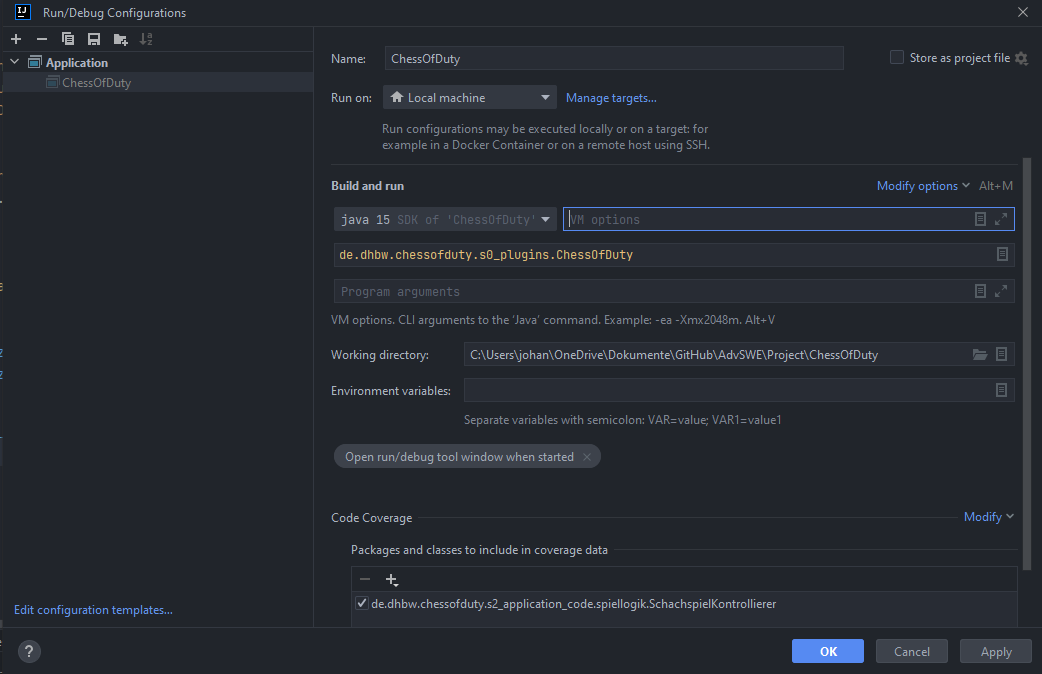
\includegraphics[scale=0.45]{Bilder/erklaerung_01.PNG}
    \captionof{figure}{Eingabefeld für VM-Options}
\end{minipage}

Sobald in das Feld Eingaben getätigt werden können, muss folgender Parameter eingetragen und gespeichert werden, bevor die Konfigurationsübersicht geschlossen und das Programm normal ausgeführt werden kann.  
\begin{figure}[h!]
    \centering
    \texttt{-Dsun.java2D.uiScale=1.0}
\end{figure}

\begin{minipage}{\linewidth}
    \centering
    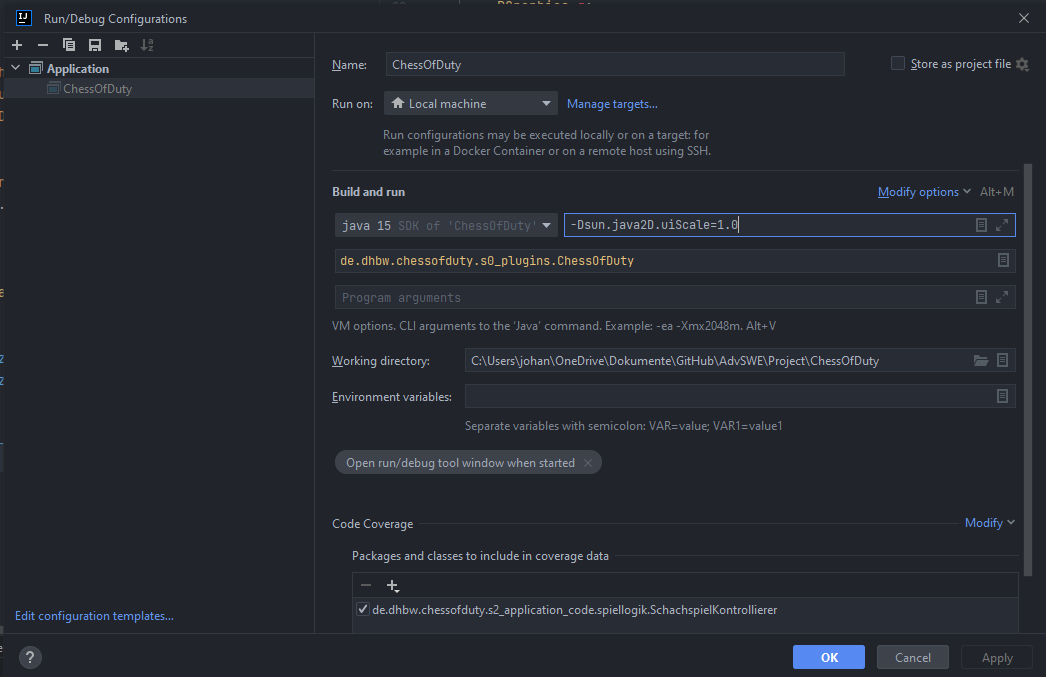
\includegraphics[scale=0.45]{Bilder/erklaerung_02.PNG}
    \captionof{figure}{VM-Options-Parameter zur richtigen Skalierung}
\end{minipage}


